\documentclass{beamer}

\usetheme{Warsaw}
\setbeamerfont*{frametitle}{size=\normalsize,series=\bfseries}
\setbeamertemplate{navigation symbols}{}
%\usefonttheme{professionalfonts}

\usepackage{listings,bera}
\usepackage[english]{babel}
\usepackage[utf8x]{inputenc}
\usepackage{times}
\usepackage[T1]{fontenc}
\usepackage{ulem}
\usepackage{listings}
\usepackage{textcomp}
\usepackage{graphicx}
\usepackage{subfigure}
\usepackage{hyperref}

%\definecolor{fore}{RGB}{249,242,215}
%\definecolor{back}{RGB}{51,51,51}
%\definecolor{title}{RGB}{255,0,90}
%\setbeamercolor{titlelike}{fg=title}
%\setbeamercolor{normal text}{fg=fore,bg=back}

\lstdefinelanguage{JavaScript}{
   keywords={attributes, class, classend, do, empty, endif, endwhile, fail, function, functionend, if, implements, in, inherit, inout, not, of, operations, out, return, set, then, types, while, use},
   keywordstyle=\color{blue}\bfseries,
   ndkeywords={},
   ndkeywordstyle=\color{yellow}\bfseries,
   identifierstyle=\color{black},
   sensitive=false,
   comment=[l]{//},
   commentstyle=\color{green}\ttfamily,
   stringstyle=\color{red}\ttfamily
}

\definecolor{keywords}{RGB}{255,0,90}
\definecolor{comments}{RGB}{60,179,113}
\definecolor{strings}{RGB}{60,179,60}
\definecolor{numbers}{RGB}{179,60,60}
\lstset{language=Python,
        extendedchars=false,
        keywordstyle=\color{keywords},
        commentstyle=\color{comments}\emph,
        stringstyle=\color{strings},
        escapechar=!
        }

% adds the \MongoLogo command to put the logo on a slide
\usepackage[absolute,overlay]{textpos}
\setlength{\TPHorizModule}{1mm}
\setlength{\TPVertModule}{1mm}
\newcommand{\MongoLogo}{
\begin{textblock}{14}(2.0,0.7)
  
\includegraphics[height=0.8cm]{logo-mongodb-ondark.png}
\end{textblock}
}

\pgfdeclareimage[height=2in]{featuregraph}{featuresPerformance.png}
\pgfdeclareimage[height=2in]{sharding}{sharding.png}

\title{Document-Oriented DBs and MongoDB}
%\subtitle{What we are and what we aren't}
\author{Mathias Stearn}
\institute{10gen}
\date{VolcaNoSQL EU -- April 20, 2010}

\AtBeginSection[]
{
  \begin{frame}<beamer>{}
    \tableofcontents[currentsection]
  \end{frame}
}


\begin{document}

\begin{frame}
  \MongoLogo
  \titlepage
\end{frame}

\begin{frame}
  \MongoLogo
  \begin{center}
    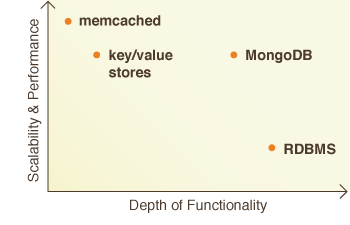
\includegraphics[height=6cm]{featuresPerformance.png}
  \end{center}
\end{frame}

\begin{frame}
  \MongoLogo
  \tableofcontents
\end{frame}

\section{Document Oriented Databases}

\begin{frame}
  \MongoLogo
  \begin{itemize}
    \item Only Two Document Oriented DBs Right Now
    \begin{itemize}
      \item MongoDB and CouchDB
      \item Everyone has an opinion on what makes a DODB
      \begin{itemize}
        \item Hard to choose ``defining'' characteristics
        \item This is my take on the space -- deal with it
      \end{itemize}
    \end{itemize}
  \end{itemize}
\end{frame}

\subsection{What they are}
\begin{frame}[fragile]
  \MongoLogo
  \begin{itemize}
    \item Document Oriented
    \begin{itemize}
      \item Think JSON Documents, not Word/OOo Documents
      \item Can store files through Attachments and GridFS
      \item Could use XML but XML sucks
    \end{itemize}
  \end{itemize}

  \begin{lstlisting}
{
  _id: "mstearn",
  name: "Mathias Stearn",
  karma: 42,
  active: true,
  birthdate: new Date(517896000000),
  interests: ["MongoDB", "Python", "!\color{strings}Üñíçøđĕ!"],
  subobjects: [{foo: "bar"},
               {foo: "baz", count: 13}]
}
  \end{lstlisting}
\end{frame}

\begin{frame}[fragile]
  \MongoLogo
  \begin{itemize}
    \item Hierarchical 
    \begin{itemize}
      \item Can nest objects to arbitrary depth
      \item Server can reach into objects
      \item Whole ``Object'' stored at one place on disk
    \end{itemize}
  \end{itemize}

  \small
  \begin{lstlisting}
{
  comments: [
    { by: 'mstearn', body: 'text', tags: ['empty']
        votes: {good: 100, bad: 10, net: 90} },
    { by: 'mdirolf', body: 'what?', tags: ['question']
        votes: {good: 30, bad: 40, net: -10} }
  ]
}
  \end{lstlisting}
\end{frame}

\subsection{What they aren't}
\begin{frame}
  \MongoLogo

  \begin{itemize}
    \item Not Relational
    \begin{itemize}
      \item Not forced into rows/columns/tables
      \item No built-in joins
      \item Less need because objects can directly store lists
      \item Many-to-Many still possible (learn how at workshop)
      \item No SQL (no SQL injections either)
      \item No Object-Relational impedance mismatch
    \end{itemize}
  \end{itemize}
\end{frame}

\begin{frame}
  \MongoLogo

  \begin{itemize}
    \item Not Just Key-Value Store
    \begin{itemize}
      \item Key and value are not separate
      \item Supports queries on non-primary keys
        \begin{itemize}
          \item Secondary Indexes
        \end{itemize}

      \item Supports Aggregation
        \begin{itemize}
          \item Currently via JavaScript MapReduce
          \item Both DBs looking into alternatives
        \end{itemize}
        
      \item Can be as fast as a KV store if you only need KV features
        \begin{itemize}
          \item But still have access to a real database when needed
        \end{itemize}

      \item Less custom code needed
    \end{itemize}
  \end{itemize}
\end{frame}

\begin{frame}
  \MongoLogo

  \begin{itemize}
    \item Not the same as stuffing a JSON blob in a database
    \begin{itemize}
      \item Database understands document format
      \item Can query on any field
      \item ``Use the right tool for the job''
    \end{itemize}
  \end{itemize}
\end{frame}

\section{CouchDB}
\begin{frame}[fragile]
  \MongoLogo

  \begin{block} {\color{red}WARNING}
    I am not an expert on CouchDB!
  \end{block}
\end{frame}

\subsection{Pros and Cons}
\begin{frame}[fragile]
  \MongoLogo

  \begin{block} {Pros}
    \begin{itemize}
      \item HTTP RESTful Interface
      \item Stores and communicates in plain JSON
      \item Query using precomputed JS Map/Reduce views
      \item Fastest if you use Bulk Insert
      \item Uses Append-Only File
    \end{itemize}
  \end{block}
\end{frame}

\begin{frame}[fragile]
  \MongoLogo

  \begin{block} {Cons}
    \begin{itemize}
      \item HTTP RESTful Interface
      \item Stores and communicates in plain JSON
      \item Query using precomputed JS Map/Reduce views
      \item Fastest if you use Bulk Insert
      \item Uses Append-Only File
    \end{itemize}
  \end{block}
\end{frame}



\section{MongoDB}
\subsection{Compared to CouchDB}
\begin{frame}[fragile]
  \MongoLogo

  \begin{block} {MongoDB}
    \begin{itemize}
      \item Custom wire protocol with many supported languages
      \item Stores and communicates in BSON (Binary JSON)
      \item Rich Ad-Hoc Query Language 
        \begin{itemize}
          \item MapReduce for aggregation
        \end{itemize}
      \item Bulk Insert available, but regular insert is very fast
      \item Data is updated in place
    \end{itemize}
  \end{block}
\end{frame}


\subsection{Into to Mongo}

\begin{frame}[fragile]
  \MongoLogo
  \begin{itemize}
    \item The Mongo Shell
      \begin{itemize}
        \item \url{http://try.mongodb.org} ${\leftarrow}$ go here now
      \end{itemize}
    \item Full JS shell + MongoDB extensions
    \item Most MongoDB documentation uses shell syntax
  \end{itemize}
\end{frame}

\begin{frame}[fragile]
  \MongoLogo

  \small
  \begin{lstlisting}[numbers=left, numberstyle=\tiny\color{red}]
db.users.insert({_id:'mstearn',
                 name: {first:'Mathias',
                        last:'Stearn'}
                 company: '10gen',
                 knows: ['MongoDB', 'Python', 'C++'],
                 posts: 42})
                 
db.users.find({_id: 'mstearn'})
db.users.find({company: '10gen'})
db.users.find({posts: {$gte: 40, $lte: 50}})
db.users.find({'name.last': 'Stearn'})
db.users.find({knows: 'MongoDB'})
db.users.find({knows: {$in: ['MongoDB', 'Mongo']}})
db.users.find({knows: {$all: ['MongoDB', 'Python']}})
db.find().sort({posts: -1}).skip(10).limit(10)
  \end{lstlisting}
\end{frame}

\subsection{Sharding}
\begin{frame}[fragile]
  \MongoLogo
  \begin{itemize}
    \item You {\tiny (probably)} don't need sharding!
    \item At the last presentation 3 out of 50 people were interested in sharding
    \item Single Master + Read Slaves for Scaling reads
    \item Largest Mongo install is 12GB
      \begin{itemize}
        \item Single Master + Replication
      \end{itemize}
    \item Wordnik.com has 1.5TB and over 5 Billion docs

    \item Speed and Scalability are different things
      \begin{itemize}
        \item But you only need scalability if you're too slow
      \end{itemize}
  \end{itemize}
\end{frame}

\subsection{JavaScript Enabled}
\begin{frame}[fragile]
  \MongoLogo
  JavaScript used for:
  \begin{itemize}
    \item Shell and Documentation
    \item (Very) Advanced Queries
    \item ``Group By'' Queries
    \item MapReduce
  \end{itemize}

  \begin{verbatim}
db.users.find({$where: "this.a + this.b >= 42"});
db.posts.group(
  { key: "user"
  , initial: {count:0, comments:0}
  , reduce: function(doc,out){
      out.count++;
      out.comments += doc.comments.length; }
  , finalize: function(out){ 
      out.avg = out.comments / out.count; }
  });
  \end{verbatim}
\end{frame}

\subsection{Fast, Scalable, Available, and Reliable}
\begin{frame}{Fast, Scalable, Available, and Reliable}
  \MongoLogo
  \begin{itemize}
  \item Master-Slave replication for Availability and Reliability
    \begin{itemize}
      \item Replica-Pairs support auto-negotiation for master
    \end{itemize}
  \item Auto-Sharding for Horizontal Scalability
    \begin{itemize}
      \item Distributes based on specified field
      \item Currently alpha
    \end{itemize}
  \item MMAP database files to automatically use available RAM
  \item Asynchronous modifications
  \end{itemize}
\end{frame}

\begin{frame}
  \MongoLogo
  \center
  \pgfuseimage{sharding}
\end{frame}

\section{What Makes Mongo Special?}

\subsection{Native Language Integration}

\begin{frame}
  \MongoLogo
  \begin{block}{Official}
    \begin{itemize}
      \item Java/JVM
      \item Python
      \item Ruby
      \item C/C++
      \item Perl
      \item PHP
    \end{itemize}
  \end{block}

  \begin{block}{Community Supported}
    Closure, 
    Scala,
    C\#,
    Haskell,
    Erlang,
    {\it and More}
  \end{block}
\end{frame}

\subsection{Rich Data Types}
\begin{frame}[fragile]
  \MongoLogo
  \begin{block}{JSON}
  \begin{itemize}
    \item String (UTF8)
    \item Double
    \item Object (hash/map/dict)
    \item Array
    \item Bool
    \item Null / Undefined
  \end{itemize}
  \end{block}

  \begin{block}{Extras}
  \begin{itemize}
    \item Date
    \item Int32 / Int64
    \item ObjectID (12 bytes: timestamp + host + pid + counter)
    \item Binary (with type byte)
  \end{itemize}
  \end{block}
\end{frame}

  
\subsection{Atomic Modifiers}
\begin{frame}[fragile]
  \MongoLogo
  \begin{itemize}
    \item \$set
    \item \$inc
    \item \$multiply (soon)
    \item \$push / \$pushAll
    \item \$pull / \$pullAll
  \end{itemize}


    \begin{small}
    \begin{verbatim}
db.posts.update({_id:SOMEID}, {$push:{tags:"mongodb"}})
db.tags.update({_id:"mongodb"}, {$inc:{count:1}},
                      {upsert:true}})
    \end{verbatim}
    \end{small}
\end{frame}

\subsection{Dynamic Queries}

\begin{frame}[fragile]
  \frametitle{Simple}
  \MongoLogo

  \begin{verbatim}
  db.posts.findOne({ user: "mstearn" });

  var cursor = db.posts.find({ user: "mstearn" });
  cursor.forEach(function(){
    doSomething(this.text);
  });
  \end{verbatim}
  
\end{frame}

\begin{frame}[fragile]
  \frametitle{Sorted}
  \MongoLogo

  \begin{verbatim}
  db.posts.find(
    { user: "mstearn" }
  ).sort({timestamp:-1})
  \end{verbatim}
  
\end{frame}
\begin{frame}[fragile]
  \frametitle{Paginated}
  \MongoLogo

  \begin{verbatim}
  db.posts.find(
    { user: "mstearn" }
  ).sort({timestamp:-1}).skip(10).limit(10);
  \end{verbatim}
  
\end{frame}
\begin{frame}[fragile]
  \frametitle{Simple Tag Search}
  \MongoLogo

  \begin{verbatim}
  db.posts.find(
    { user: "mstearn"
    , tags: "mongo"
    }
  ).sort({timestamp:-1}).skip(10).limit(10);
  \end{verbatim}
  
\end{frame}

\begin{frame}[fragile]
  \frametitle{Complex Tag Search}
  \MongoLogo

  \begin{verbatim}
  db.posts.find(
    { user: "mstearn"
    , tags: {$in: ["mongo", "mongodb"]}
    }
  ).sort({timestamp:-1}).skip(10).limit(10);
  \end{verbatim}
  
\end{frame}

\begin{frame}[fragile]
  \frametitle{Nested Objects}
  \MongoLogo

  \begin{verbatim}
  db.posts.find(
    { user: "mstearn"
    , tags: {$in: ["mongo", "mongodb"]}
    , comments.user: "mdirolf"
    }
  ).sort({timestamp:-1}).skip(10).limit(10);
  \end{verbatim}
  
\end{frame}
\begin{frame}[fragile]
  \frametitle{Regular Expressions}
  \MongoLogo

  \begin{verbatim}
  db.posts.find(
    { user: "mstearn"
    , tags: {$in: ["mongo", "mongodb"]}
    , comments.user: "mdirolf"
    , text: /windows/i
    }
  ).sort({timestamp:-1}).skip(10).limit(10);
  \end{verbatim}
  
\end{frame}
\begin{frame}[fragile]
  \frametitle{Ranges}
  \MongoLogo

  \begin{verbatim}
  db.posts.find(
    { user: "mstearn"
    , tags: {$in: ["mongo", "mongodb"]}
    , comments.user: "mdirolf"
    , text: /windows/i
    , points: {$gt: 10, $lt: 100}
    }
  ).sort({timestamp:-1}).skip(10).limit(10);
  \end{verbatim}
  
\end{frame}
\begin{frame}[fragile]
  \frametitle{Arbitrary JavaScript}
  \MongoLogo

  \begin{verbatim}
  db.posts.find(
    { user: "mstearn"
    , tags: {$in: ["mongo", "mongodb"]}
    , comments.user: "mdirolf"
    , text: /windows/i
    , points: {$gt: 10, $lt 100}
    , $where: "this.a + this.b >= 42"
    }
  ).sort({timestamp:-1}).skip(10).limit(10);
  \end{verbatim}
\end{frame}


\section{MapReduce}

\subsection{Built-In MapReduce}
\begin{frame} [fragile]
  \MongoLogo

  \begin{small}
  \begin{verbatim}
db.posts.mapReduce(
   function() {
     this.comments.forEach(c){
       emit(c.user, 
            {count:1, words:c.text.split().length; } }
 , function(key, values){
     for (var i=1; i<values.length; i++){
       values[0].count += values[i].count;
       values[0].words += values[i].words; }
     return values[0]; }
 , { finalize: function(out){
       out.avg = out.words / out.count;
       return out; }
   , query: {posted: {$gt: new Date(2010,0,1)}}
   , out: 'posts.comment_stats'
   }
 });
  \end{verbatim}
  \end{small}
\end{frame}


\subsection{Easy Hadoop-Mongo Integration}
\begin{frame}{Easy Hadoop-Mongo Integration}
  \MongoLogo

  \begin{itemize}
    \item mongoexport can export to JSON/CSV/TSV
      \begin{itemize}
        \item Can also easily use a custom script
      \end{itemize}
    \item Process in Hadoop
    \item Use mongoimport to get data back into MongoDB
  \end{itemize}

\end{frame}


\subsection{Better Hadoop-Mongo Integration}
\begin{frame} {Better Hadoop-Mongo Integration}
  \MongoLogo

  \begin{itemize}
    \item mongodump writes a stream of BSON to a file
    \item Write an InputFilter and RecordReader to read BSON
    \item Write a BSONWriter class to directly use the data
      \begin{itemize}
        \item Just added two methods to driver to make this easier
      \end{itemize}
    \item Process the data with the Java/Scala/Closure driver
    \item Write a custom RecordWriter to either:
      \begin{itemize}
        \item Dump to a file and use mongorestore
        \item Dump the output directly to MongoDB
      \end{itemize}
    \item Optional: use renameCollection to mimic our MapReduce
  \end{itemize}

\end{frame}

\section{}

\begin{frame}{Upcoming events}{}
  \MongoLogo

  \begin{itemize}
    \item NoSQL Live! from Boston (March 11)
    \item MongoDB Training in San Francisco (March 25)
    \item San Fransisco MySQL Meetup (April 12)
  \end{itemize}
\end{frame}

\begin{frame}{Links}{}
  \MongoLogo

  \begin{itemize}
    \item http://mongo.kylebanker.com (Try mongo in your browser)
    \item http://www.mongodb.org
    \item \#mongodb on irc.freenode.net
    \item mongodb-user on google groups
  \end{itemize}
  \begin{itemize}
    \item mathias@10gen.com
    \item @mathias\_mongo on twitter
  \end{itemize}
\end{frame}

\end{document}

% vim: set softtabstop=2
